%
% % % \usepackage{booktabs}
% \newcommand{\ra}[1]{\renewcommand{\arraystretch}{#1}}
% \begin{table*}\centering
%
% % \resizebox{100}
% \begin{tabular}{@{}rrrrcrrrcrrr@{}}\toprule
% & \multicolumn{3}{c}{$w = 8$} & \phantom{abc}& \multicolumn{3}{c}{$w = 16$} &
% \phantom{abc} & \multicolumn{3}{c}{$w = 32$}\\
% \cmidrule{2-4} \cmidrule{6-8} \cmidrule{10-12}
% & $t=0$ & $t=1$ & $t=2$ && $t=0$ & $t=1$ & $t=2$ && $t=0$ & $t=1$ & $t=2$\\ \midrule
% $dir=1$\\
% $c$ & 0.0790 & 0.1692 & 0.2945 && 0.3670 & 0.7187 & 3.1815 && -1.0032 & -1.7104 & -21.7969\\
% $c$ & -0.8651& 50.0476& 5.9384&& -9.0714& 297.0923& 46.2143&& 4.3590& 34.5809& 76.9167\\
% $c$ & 124.2756& -50.9612& -14.2721&& 128.2265& -630.5455& -381.0930&& -121.0518& -137.1210& -220.2500\\
% $dir=0$\\
% $c$ & 0.0357& 1.2473& 0.2119&& 0.3593& -0.2755& 2.1764&& -1.2998& -3.8202& -1.2784\\
% $c$ & -17.9048& -37.1111& 8.8591&& -30.7381& -9.5952& -3.0000&& -11.1631& -5.7108& -15.6728\\
% $c$ & 105.5518& 232.1160& -94.7351&& 100.2497& 141.2778& -259.7326&& 52.5745& 10.1098& -140.2130\\
% \bottomrule
% \end{tabular}
% \caption{Caption}
% \end{table*}



%
% \setlength\LTleft{-1in}
% \setlength\LTright{-1in}
% % \begin{longtable}{@{\extracolsep{\fill}}*{13}{|r}|@{}}
% %
% %
% %
% \begin{longtable}{lrrrcrrrr}
% \toprule
% %
% & \multicolumn{3}{c}{including time costs} & \phantom{a}& \multicolumn{4}{c}{excluding time costs} \\
% \cmidrule{2-4} \cmidrule{6-9}
% %
% %
% % & \multicolumn{2}{c}{VRPTT} &\multicolumn{2}{c}{VRPTTMU} &
% % \phantom{abc} & \multicolumn{2}{c}{VRPTT} &\multicolumn{2}{c}{VRPTTMU} \\
% %
% instance &  VRPTT &  VRPTTMU &  OPT\_TTRP &&  VRPTT &  VRPTTMU &  LB\_VRPTT &  UB\_VRPTT \\
% %




\appendix

\section{Symbols and Abbreviations}


Many symbols and abbreviations are used throughout this thesis.
They are enumerated with their meaning in Table \ref{tab:symbols}.

% \begin{}[!h]
% \centering
% \caption{Symbols and abbreviations with their meanings.}
% \label{tab:symbols}
\setlength\LTleft{-1.1in}
\setlength\LTright{-2in}
\begin{longtable}{ll}

\toprule
Symbol       & Meaning       \\ \midrule \endhead
VRP & The vehicle routing problem. \\
RVRP & The rich vehicle routing problem. \\
VRPMS & The vehicle routin problem with multiple synchronization constraints. \\
VRPTT & The vehicle routing problem with trailers and transshipments. \\
VRPTTMU & The vehicle routing problem with trailers, transshipments and multiple unloads. \\

\includegraphics[width=.04\textwidth]{img/lorry_icon.pdf} & The  lorry icon. \\

\includegraphics[width=.04\textwidth]{img/trailer_icon.pdf} & The trailer icon. \\

\includegraphics[width=.04\textwidth]{img/couple_vertex.pdf} & The transshipment couple vertex icon. \\

\includegraphics[width=.04\textwidth]{img/decouple_vertex.pdf} & The transshipment decouple vertex icon. \\

\includegraphics[width=.04\textwidth]{img/supply_vertex.pdf} & The  supply collection vertex icon.\\

\includegraphics[width=.04\textwidth]{img/time-window_icon.pdf} & The time window icon. \\

\includegraphics[width=.04\textwidth]{img/vehicle_start.pdf} & The start of vehicle path vertex icon. \\

\includegraphics[width=.04\textwidth]{img/vehicle_end.pdf} & The end of vehicle path vertex icon.\\

\includegraphics[width=.04\textwidth]{img/transshipment_location_icon.pdf} & The transshipment location icon.\\

\includegraphics[width=.04\textwidth]{img/customer_location_icon.pdf} & The customer icon. \\

\includegraphics[width=.04\textwidth]{img/depot_location_icon.pdf} & The depot icon.\\

\includegraphics[width=.04\textwidth]{img/super_source_icon.pdf} & The supersource vertex icon. \\

\includegraphics[width=.04\textwidth]{img/super_sink_icon.pdf} & The supersink vertex icon.\\
$\mathcal L$ & The set of locations. \\
$\mathcal D$ & The mapping from a pair of locations to the distance between them. \\
$\mathcal F$ & The set of vehicles in the fleet. \\
$\mathcal L^{\rm types}$ & The set of location types. \\
$locationType_i$ & The location type of location $i$. \\
$\alpha_i$ & The start of the time window of location $i$. \\
$\beta_i$ & The end of the time window of location $i$. \\
$\mathcal L^{\rm customer}$ & The set of customer locations. \\
$locationSupply_i$ & The supply of customer location $i$. \\
$\mathcal F^{\rm types}$ & The set of vehicle types. \\
$\mathcal F^{\rm lorry}$ & The set of vehicle lorries. \\
$\mathcal F^{\rm trailer}$ & The set of trailers. \\
$\mathcal F^{\rm axle-types}$ & The set of axle types of vehicles.\\
$f^{\rm type}_k$ & The vehicle type of  vehicle $k$. \\
$f^{\rm capacity}_k$ & The capacity of vehicle $k$. \\
$f^{\rm fixed}_k$ & The fixed cost of vehicle $k$. \\
$f^{\rm distance}_k$ & The variable distance cost of vehicle $k$ per kilometer. \\
$f^{\rm time}_k$ & The variable time cost of vehicle $k$ per hour. \\
$f^{\rm axle-type}_k$ & The axle type of vehicle $k$. \\
$f^{\rm speed}_k$ & The maximum speed of vehicle $k$ on distances longer than $\phi$. \\
$f^{\rm shortspeed}_k$ & The maximum speed of vehicle $k$ on distances shorter than or equal to $\phi$. \\
$f^{\rm loadspeed}_k$ & The load speed of lorry $k$ in minutes per unit. \\
$\phi$ & The cut-off distance that determines the maximum speed of the vehicles. \\
$\tau^{\rm D}$ & The duration of coupling or decoupling a trailer at the depot in minutes. \\
$\tau^{\rm R}$ & The duration of coupling or decoupling a trailer at a transshipment location in minutes. \\
$\mathcal R^-$ & The set of transshipment decouple vertices. \\
$\mathcal R^+$ & The set of transshipment couple vertices. \\
$\mathcal L^{\rm transshipment}$ & The set of transshipment locations. \\
$r^{j,-}_m$ & The decouple vertex of the $m$th transshipment vertex pair  at transshipment location $j$. \\
$r^{j,+}_m$ & The couple vertex of transshipment vertex pair $m$ at transshipment location $j$. \\
$\eta$ & The amount of transshipment vertex pairs per transshipment location. \\
$\mathcal S$ & The set of the customers' supply collection vertices \\
$s_i$ & the supply collection vertex of customer location $i$. \\
$\mathcal S^{\rm trailer}$ & The set of supply collection vertices of the the trailer customers.  \\
$\mathcal S^{\rm lorry}$ & The set of supply collection vertices of the lorry customers. \\
$\mathcal M^-$ & The set of end vertices of the lorries.\\
$\mathcal M^+$ & The set of start vertices of the lorries. \\
$m^-_k$ & The end vertex of lorry $k$. \\
$m^+_k$ & The start vertex of lorry $k$. \\
$\mathcal N^-$ & The set of end vertices of the trailers.\\
$\mathcal N^+$ & The set of start vertices of the trailers. \\
$n^-_l$ & The end vertex of trailer $l$. \\
$n^+_l$ & The start vertex of trailer $l$. \\
$\mathcal V$ & The union of the set of vehicle start and end vertices, the set of transshipment decouple \\
& and couple vertices and the set of customer supply collection vertices.  \\
$v^{\rm loc} $ & The location of vertex $v$. \\
$\tau^{\rm start}_v $ & The start of vertex $v$'s time window. \\
$\tau^{\rm end}_v $ & The end of vertex $v$'s time window. \\
$\tau^{\rm min} $ & The start of the time horizon. \\
$\tau^{\rm max} $ & The end of the time horizon. \\
$\delta_{u,v} $ & The distance between vertex $u$ and $v$. \\
% $\epsilon^{\phi}_i$ & the set of vertices distanced less than $\phi$ from vertex $i$ \\
$\tau^{\rm travel}_{u,v,k} $ & The travel time of vehicle $k$ between vertices $u$ and $v$.\\
$\tau^{\rm extra}_{u,v,k,l} $ & The extra time it takes for lorry $l$ to traverse edge $(u,v)$ if it is \\
&  coupled with trailer $l$. \\
$travelTime$ & The function that takes as input an edge and a path assignment and returns the amount of time \\
&  it took for vehicles to traverse that edge.\\
$visitationStart$ & The function that takes as input a vertex, a path assignment and a time table and \\
& returns the time at which the the vertex' visitation started. \\
$\mathcal E $ & The set of edges $ \{ (u,v): u,v \in \mathcal V , u \neq v \} $. \\
$\mathcal G $ & The graph $ (\mathcal V, \mathcal E) $. \\
$x^k_{u,v}$ & The binary decision variable that models whether lorry $k$ traverses edge $(u,v)$. \\
$y^{k,l}_{u,v}$ & T`he binary decision variable that models whether lorry $k$ traverses edge $(u,v)$ \\
& whilst coupled to trailer $l$. \\
$t^k_{u,v}$ & The real-valued decision variable that models at which time lorry $k$ finishes traversing edge $(u,v)$. \\
$z^k_{u,v}$ & The real-valued decision variable that models the amount of load with which \\
&   vehicle $k$ traverses edge $(u,v)$. \\
% $ X$ & $ (x^k_{u,v}) \text{ for } k \in  \mathcal F^{\rm lorry}, u,v \in \mathcal V$ \\
% $ Y$ & $ (y^{k,l}_{u,v}) \text{ for } k \in  \mathcal F^{\rm lorry} ,
% \l  \in  \mathcal F^{\rm trailer}, u,v \in \mathcal V$ \\
% $ T $&$ (t^k_{u,v}) $ for $ k \in  \mathcal F^{\rm lorry}, u,v \in \mathcal V$ \\
% $ L $&$ (z^k_{u,v}) $ for $ k \in  \mathcal F, u,v \in \mathcal V$ \\
$C$ & The objective function. \\
$C^{\rm distance}$ & The function that calculates the distance-related costs of a solution. \\
$C^{\rm time}$ & The function that calculates the time-related costs of a solution. \\
$C^{\rm fixed}$ & The function that calculates the fixed costs of a solution. \\
$X$ & The lorries' paths of a solution.  \\
$Y$ & The trailers' paths of a solution.\\
$T$ & The time table of a solution.\\
$L$ & The load table of a solution.\\
$XY$ & The path assignment $(X,Y)$. \\
VNS & The variable neighborhood search . \\
$\omega^{\rm unserved-customer} $ & The penalty for not serving a  customer.  \\
$U^{\rm unserved-customer} $ & The function that calculates the penalty of a solution due to unserved customers. \\
$\omega^{\rm lorry-customer} $ & The penalty for visiting a lorry customer with a trailer. \\
$U^{\rm lorry-customer} $ & The function that calculates the penalty of a solution due to lorry customers visited with trailers. \\
$\omega^{\rm time-window} $ & The penalty per minute for a lorry violating the end of a vertex' time window. \\
$U^{\rm time-window} $ & The function that calculates the penalty of a solution due to violated time windows. \\
$\omega^{\rm capacity-shortage} $ & The penalty per supply unit left uncollected of a visited customer. \\
$U^{\rm capacity-shortage} $ & The function that calculates the penalty of a solution due to uncollected supply of \\
&  visited customers. \\
$U$ & The functional that calculates the penalty of a solution. \\
% $\mathcal O$ & The set of neighborhood operators. \\
$nSamples$ & The amount of path assignments that the operation $merge lorries$ returns. \\
$\mathcal G^{\rm c}$ & The capacity graph $(\mathcal V^{\rm c},\mathcal E^{\rm c})$. \\
$\mathcal V^{\rm c}$ & The set of vertices of the capacity graph $\mathcal G^{\rm c}$. \\
$\mathcal E^{\rm c}$ & The set of edges of the capacity graph $\mathcal G^{\rm c}$.\\
$capacity $ & A mapping from edges in the capacity graph to their capacities. \\
$\mathcal P$ & The set of vertices used to model load transfers to trailers when constructing the load table.  \\
$p_l$ & The vertex used to model load transfers to trailer $l$ when constructing the load table. \\
$source $ & The vertex used as a supersource when constructing the time and load table. \\
$sink $ & The vertex used as a supersink when constructing the time and load table. \\
$f^{\rm c} $ & A mapping that represent the solution to the maximum flow problem on the capacity graph \\
& from the supersource to the supersink.   \\
$|f^{\rm c}| $ & The total amount of customer supply collected. \\
$\mathcal G^{\rm trailer}$ & The graph $(\mathcal V$ used to determine trailers' trailer paths. \\
$trailerPath_l$ & The trailer path of trailer $l$ which is used to determine the load of a trailer during \\
& each edge it traverses. \\
$\mathcal E^{\rm pair}$  & The set of edges that connects each transshipment decouple vertex with the \\
& couple  vertex it is paired with.  \\
$\mathcal E^{\rm used-trailer}$  & The set of edges traversed by any trailer.  \\
$\mathcal V^{\rm precedence}$ & The set of vertices used to model the precedence graph. \\
$\mathcal E^{\rm earliest}$ & The set of edges used to calculate the earliest arrival times. \\
$\mathcal E^{\rm latest}$ & The set of edges used to calculate the latest time at which trailers start can start their paths.  \\
$duration^{\rm earliest}$ & A function that maps from edges to their weights. \\
$duration^{\rm latest}$ & A function that maps from edges to their weights. \\
$duration^{\rm result}$ & A function that maps from edges to their weights. \\
$\mathcal G^{\rm earliest}$ & $(\mathcal V^{\rm precedence},\mathcal E^{\rm earliest},duration^{\rm earliest} )$ \\
$\mathcal G^{\rm latest}$ & $(\mathcal V^{\rm precedence},\mathcal E^{\rm latest},duration^{\rm latest} )$ \\
$\mathcal G^{\rm result}$ & $(\mathcal V^{\rm precedence},\mathcal E^{\rm earliest},duration^{\rm result} )$ \\
$\mathcal V^{\rm start}$ & The set of edges used to model the start of vertex visits in a precedence graph. \\
$\mathcal V^{\rm end}$ & The set of edges used to model the end of vertex visits in a precedence graph. \\
$\mathcal E^{\rm latest-start}$ & The set of edges used to constrain the time at which lorries start their paths. \\
$score$ & The function that calculates the score of a solution, which is the sum of its costs \\
&  and its penalties. \\
$TABU$ & The collection that is used to cache path assignments. \\
$PQ$ & The collection that keeps solutions with unexplored neighborhoods in sorted order. \\
$p$ & The probability that a random item is removed from the $PQ$ instead the one  \\
& with the highest priority. \\
$VRPTT\_UB$ & Upper bounds for the VRPTT excluding time costs. \\
$VRPTT\_LB$ & Lower bounds for the VRPTT excluding time costs. \\
$TTRP\_OPT$ & The optimal values for the TTRP including time costs. \\

% $trailerPath_l$ & the sequence of vertices visited by vehicle $k$ \\
\bottomrule
\caption{Symbols and abbreviations with their meanings.}
\label{tab:symbols}
\end{longtable}


% \begin{figure}[!ht]
%   \centering
%     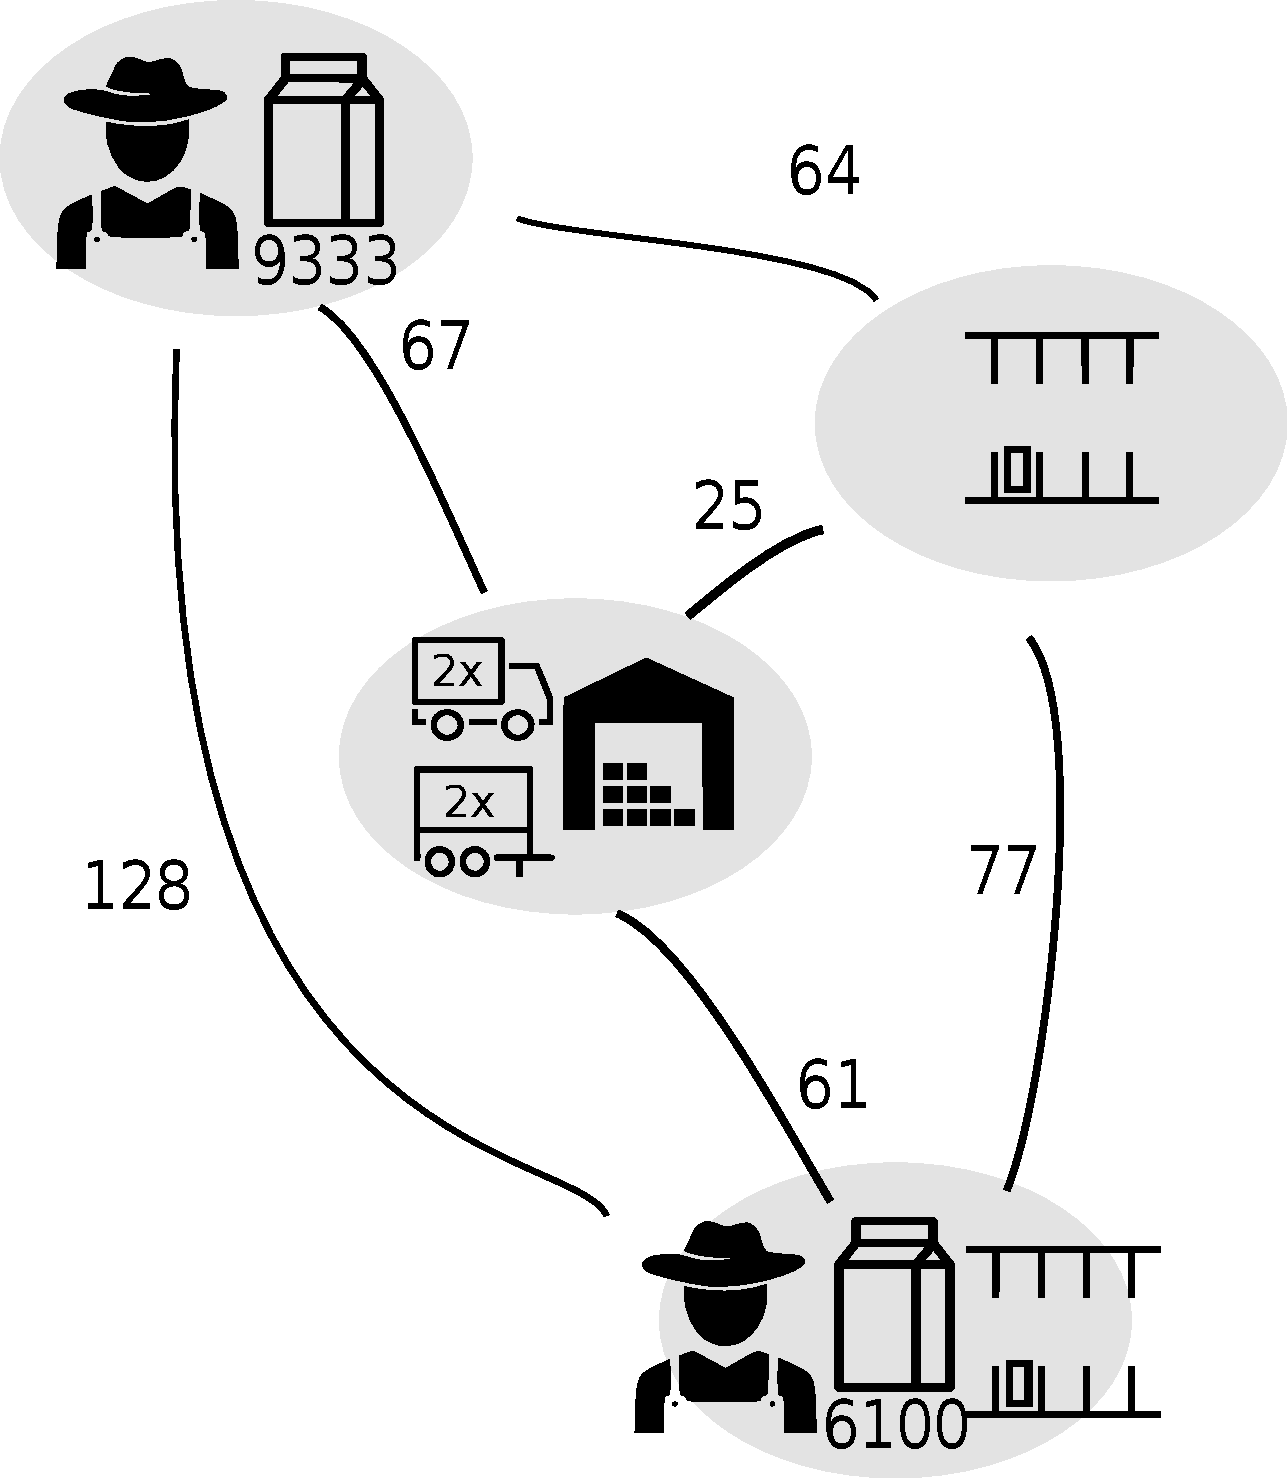
\includegraphics[width=.8\textwidth]{img/1_1_1_4.pdf}
% \end{figure}

\section{Results and Bounds}
\subsection{Nominal Values}
\label{sec:bounds}

Table \ref{tab:nominal} describes for each instance the lowest cost solution found by the VNS for the VRPTT and the VRPTTMU  and  the optimal value for the TTRP provided in \cite{drexl2011branch} which include time costs  and the lower and upper bound of the VRPTT provided in ~\cite{drexl2014bandc} which exclude time costs.




%
\setlength\LTleft{-1in}
\setlength\LTright{-1in}
% \begin{longtable}{@{\extracolsep{\fill}}*{13}{|r}|@{}}
%
%
%
\begin{longtable}{lrrrcrrrr}
\toprule
%
& \multicolumn{3}{c}{including time costs} & \phantom{a}& \multicolumn{4}{c}{excluding time costs} \\
\cmidrule{2-4} \cmidrule{6-9}
%
%
% & \multicolumn{2}{c}{VRPTT} &\multicolumn{2}{c}{VRPTTMU} &
% \phantom{abc} & \multicolumn{2}{c}{VRPTT} &\multicolumn{2}{c}{VRPTTMU} \\
%
instance &  VRPTT &  VRPTTMU &  OPT\_TTRP &&  VRPTT &  VRPTTMU &  LB\_VRPTT &  UB\_VRPTT \\
%
\midrule \endhead
1\_1\_1\_00      &     32660.0 &       32660.0 &        32480.0 &&       25280.0 &         25280.0 &          25280.0 &          25280.0 \\
1\_1\_1\_01      &     43440.0 &       42080.0 &        43260.0 &&       32040.0 &         29960.0 &          32040.0 &          32040.0 \\
1\_1\_1\_02      &     40200.0 &       40200.0 &        40020.0 &&       30360.0 &         30360.0 &          30360.0 &          30360.0 \\
1\_1\_1\_03      &     39030.0 &       39030.0 &        38850.0 &&       29730.0 &         29730.0 &          29730.0 &          29730.0 \\
1\_1\_1\_04      &     58467.0 &       50840.0 &        58993.0 &&       39567.0 &         34640.0 &          39575.0 &          39575.0 \\
1\_1\_1\_05      &     36960.0 &       35030.0 &        36900.0 &&       28680.0 &         26450.0 &          28680.0 &          28680.0 \\
1\_1\_1\_06      &     47695.0 &       47695.0 &        47515.0 &&       33535.0 &         33535.0 &          33535.0 &          33535.0 \\
1\_1\_1\_07      &     41450.0 &       41450.0 &        41270.0 &&       31130.0 &         31130.0 &          31130.0 &          31130.0 \\
1\_1\_1\_08      &     37140.0 &       37140.0 &        36960.0 &&       28680.0 &         28680.0 &          28680.0 &          28680.0 \\
1\_1\_1\_09      &     48065.0 &       48065.0 &        47885.0 &&       33665.0 &         33665.0 &          33665.0 &          33665.0 \\
1\_1\_1\_10      &     39540.0 &       39540.0 &        39900.0 &&       29040.0 &         29040.0 &          29117.0 &          29117.0 \\
1\_1\_1\_11      &     37428.0 &       37428.0 &        37852.0 &&       28128.0 &         28128.0 &          28205.0 &          28205.0 \\
1\_1\_1\_12      &     48860.0 &       45840.0 &        48680.0 &&       35120.0 &         32040.0 &          35120.0 &          35120.0 \\
1\_1\_1\_13      &     38422.0 &       38422.0 &        38878.0 &&       28582.0 &         28582.0 &          28659.0 &          28659.0 \\
1\_1\_1\_14      &     46631.0 &       46560.0 &        47069.0 &&       32882.0 &         32040.0 &          32890.0 &          32890.0 \\
1\_1\_1\_15      &     45450.0 &       45450.0 &        45270.0 &&       32430.0 &         32430.0 &          32430.0 &          32430.0 \\
1\_1\_1\_16      &     30420.0 &       30420.0 &        30240.0 &&       24240.0 &         24240.0 &          24240.0 &          24240.0 \\
1\_1\_1\_17      &     43724.0 &       40070.0 &        44016.0 &&       31364.0 &         28790.0 &          31372.0 &          31372.0 \\
1\_1\_1\_18      &     67855.0 &       56400.0 &        68445.0 &&       44635.0 &         37500.0 &          44643.0 &          44643.0 \\
1\_1\_1\_19      &     36220.0 &       36220.0 &        36100.0 &&       28120.0 &         28120.0 &          28120.0 &          28120.0 \\
1\_1\_1\_20      &     48310.0 &       42130.0 &        48610.0 &&       33850.0 &         29830.0 &          33858.0 &          33858.0 \\
1\_1\_1\_21      &     40020.0 &       37280.0 &        39840.0 &&       30360.0 &         27620.0 &          30360.0 &          30360.0 \\
1\_1\_1\_22      &     42610.0 &       42610.0 &        42430.0 &&       31690.0 &         31690.0 &          31690.0 &          31690.0 \\
1\_1\_1\_23      &     50350.0 &       47590.0 &        50170.0 &&       35890.0 &         32950.0 &          35890.0 &          35890.0 \\
1\_1\_1\_24      &     44180.0 &       41780.0 &        44000.0 &&       32493.0 &         29960.0 &          32501.0 &          32501.0 \\
1\_1\_1\_25      &     52700.0 &       49570.0 &        53380.0 &&       36440.0 &         33730.0 &          36448.0 &          36448.0 \\
1\_1\_1\_26      &     44510.0 &       42660.0 &        44330.0 &&       32810.0 &         30480.0 &          32810.0 &          32810.0 \\
1\_1\_1\_27      &     42100.0 &       42100.0 &        41980.0 &&       31480.0 &         30870.0 &          31480.0 &          31480.0 \\
1\_1\_1\_28      &     33800.0 &       31320.0 &        33620.0 &&       26720.0 &         24240.0 &          26720.0 &          26720.0 \\
1\_1\_1\_29      &     45740.0 &       43590.0 &        45560.0 &&       33440.0 &         30870.0 &          33440.0 &          33440.0 \\
2\_2\_2\_00      &     56280.0 &       54220.0 &        55980.0 &&       39180.0 &         36460.0 &          39180.0 &          39180.0 \\
2\_2\_2\_01      &     74787.0 &       56290.0 &        75193.0 &&       56007.0 &         38007.0 &          56084.0 &          56084.0 \\
2\_2\_2\_02      &     65742.0 &       56720.0 &        65180.0 &&       43122.0 &         38900.0 &          43217.0 &          43217.0 \\
2\_2\_2\_03      &     71718.0 &       53798.0 &        71298.0 &&       55338.0 &         37418.0 &          55420.0 &          55420.0 \\
2\_2\_2\_04      &     56709.0 &       54171.0 &        56409.0 &&       38169.0 &         36871.0 &          38252.0 &          38252.0 \\
2\_2\_2\_05      &     42260.0 &       41890.0 &        41960.0 &&       31340.0 &         29830.0 &          31340.0 &          31340.0 \\
2\_2\_2\_06      &     71444.0 &       66230.0 &        71084.0 &&       45966.0 &         42830.0 &          45974.0 &          45974.0 \\
2\_2\_2\_07      &     85527.0 &       56775.0 &        86251.0 &&       61647.0 &         37474.0 &          59499.0 &          59499.0 \\
2\_2\_2\_08      &     72580.0 &       72580.0 &        72340.0 &&       48280.0 &         47250.0 &          48280.0 &          48280.0 \\
2\_2\_2\_09      &     80945.0 &       62945.0 &        81275.0 &&       59105.0 &         41105.0 &          59182.0 &          59182.0 \\
2\_2\_2\_10      &     75040.0 &       55040.0 &        74740.0 &&       57640.0 &         37640.0 &          57640.0 &          57640.0 \\
2\_2\_2\_11      &     82157.0 &       64157.0 &        82493.0 &&       59897.0 &         41897.0 &          59974.0 &          59974.0 \\
2\_2\_2\_12      &     67055.0 &       63400.0 &        67125.0 &&       43655.0 &         41660.0 &          43728.0 &          43728.0 \\
2\_2\_2\_13      &     56122.0 &       54510.0 &        55702.0 &&       38302.0 &         37350.0 &          38314.0 &          38314.0 \\
2\_2\_2\_14      &     58264.0 &       50150.0 &        53438.0 &&       38884.0 &         35330.0 &          38026.0 &          38026.0 \\
2\_2\_2\_15      &     55428.0 &       52220.0 &        55068.0 &&       38792.0 &         35550.0 &          38877.0 &          38877.0 \\
2\_2\_2\_16      &    105591.0 &       84520.0 &       104160.0 &&       72891.0 &         53880.0 &          72968.0 &          72968.0 \\
2\_2\_2\_17      &     63456.0 &       60820.0 &        62976.0 &&       41796.0 &         41140.0 &          41891.0 &          41891.0 \\
2\_2\_2\_18      &     49750.0 &       48145.0 &        49450.0 &&       35470.0 &         33145.0 &          35470.0 &          35470.0 \\
2\_2\_2\_19      &     66033.0 &       62140.0 &        65613.0 &&       43653.0 &         41270.0 &          43665.0 &          43665.0 \\
2\_2\_2\_20      &     61099.0 &       60050.0 &        60739.0 &&       40639.0 &         39710.0 &          40799.0 &          40799.0 \\
2\_2\_2\_21      &     44870.0 &       44145.0 &        44570.0 &&       32810.0 &         31065.0 &          32810.0 &          32810.0 \\
2\_2\_2\_22      &     53920.0 &       53920.0 &        53620.0 &&       37780.0 &         37780.0 &          37780.0 &          37780.0 \\
2\_2\_2\_23      &     84051.0 &       66051.0 &        83691.0 &&       61491.0 &         43491.0 &          61574.0 &          61574.0 \\
2\_2\_2\_24      &     80947.0 &       62947.0 &        80527.0 &&       59707.0 &         41454.0 &          59790.0 &          59790.0 \\
2\_2\_2\_25      &     69843.0 &       65850.0 &        69363.0 &&       45363.0 &         44010.0 &          45458.0 &          45458.0 \\
2\_2\_2\_26      &     49050.0 &       46650.0 &        48810.0 &&       35190.0 &         32430.0 &          35190.0 &          35190.0 \\
2\_2\_2\_27      &     59522.0 &       55810.0 &        59102.0 &&       40368.0 &         37045.0 &          40380.0 &          40380.0 \\
2\_2\_2\_28      &     69097.0 &       66330.0 &        68737.0 &&       45397.0 &         43675.0 &          45409.0 &          45409.0 \\
2\_2\_2\_29      &     85435.0 &       67435.0 &        85135.0 &&       61615.0 &         43615.0 &          61698.0 &          61698.0 \\
3\_3\_3\_00      &     78232.0 &       70890.0 &        75172.0 &&       49672.0 &         44910.0 &          48033.0 &          48033.0 \\
3\_3\_3\_01      &     73197.0 &       64970.0 &        72597.0 &&       47037.0 &         42180.0 &          47061.0 &          47061.0 \\
3\_3\_3\_02      &    107945.0 &       96850.0 &       106984.0 &&       75202.0 &         57910.0 &          71290.7 &          75209.0 \\
3\_3\_3\_03      &     58361.0 &       55840.0 &        58659.0 &&       39461.0 &         37240.0 &          39469.0 &          39469.0 \\
3\_3\_3\_04      &     64572.0 &       60940.0 &        64032.0 &&       43872.0 &         41140.0 &          43880.0 &          43880.0 \\
3\_3\_3\_05      &    110244.0 &       93283.0 &       108285.0 &&       75144.0 &         56623.0 &          64918.2 &          75464.0 \\
3\_3\_3\_06      &     86800.0 &       77154.0 &        86260.0 &&       63940.0 &         48714.0 &          64018.0 &          64018.0 \\
3\_3\_3\_07      &     81330.0 &       70134.0 &        80850.0 &&       60930.0 &         44154.0 &          60930.0 &          60930.0 \\
3\_3\_3\_08      &     98000.0 &       79529.0 &        98388.0 &&       69610.0 &         48929.0 &          66850.6 &          68676.0 \\
3\_3\_3\_09      &     95352.0 &       68149.0 &        87091.0 &&       67092.0 &         42440.0 &          59008.7 &          61207.0 \\
3\_3\_3\_10      &     93029.0 &       73160.0 &        92740.0 &&       66914.0 &         47720.0 &          66940.0 &          66940.0 \\
3\_3\_3\_11      &     81927.0 &       62910.0 &        81336.0 &&       60807.0 &         41490.0 &          60344.0 &          60344.0 \\
3\_3\_3\_12      &     65993.0 &       60910.0 &        65857.0 &&       42953.0 &         40815.0 &          42961.0 &          42961.0 \\
3\_3\_3\_13      &     68244.0 &       65535.0 &        68506.0 &&       44563.0 &         42375.0 &          44648.0 &          44648.0 \\
3\_3\_3\_14      &    102645.0 &       89160.0 &       100560.0 &&       70845.0 &         53880.0 &          68338.0 &          69527.0 \\
3\_3\_3\_15      &    105995.0 &       90583.0 &       105626.0 &&       72670.0 &         55423.0 &          69275.3 &          72680.0 \\
3\_3\_3\_16      &     80811.0 &       61561.0 &        80391.0 &&       59391.0 &         40621.0 &          59133.1 &          59403.0 \\
3\_3\_3\_17      &     96331.0 &       83732.0 &        95971.0 &&       69211.0 &         51150.0 &          67813.0 &          69353.0 \\
3\_3\_3\_18      &     73548.0 &       70662.0 &        73008.0 &&       47628.0 &         45942.0 &          47640.0 &          47640.0 \\
3\_3\_3\_19      &     90797.0 &       73150.0 &        90790.0 &&       64637.0 &         46244.0 &          61289.6 &          64578.0 \\
3\_3\_3\_20      &     99197.0 &       91090.0 &        93265.0 &&       69617.0 &         64690.0 &          65981.0 &          66840.0 \\
3\_3\_3\_21      &    117307.0 &      102810.0 &       115094.0 &&       80467.0 &         61290.0 &          73564.2 &          78791.0 \\
3\_3\_3\_22      &    113547.0 &       99160.0 &       107303.0 &&       76824.0 &         59920.0 &          69179.4 &          74467.0 \\
3\_3\_3\_23      &     80213.0 &       60320.0 &        79900.0 &&       60473.0 &         40580.0 &          60473.0 &          60473.0 \\
3\_3\_3\_24      &    101044.0 &       78849.0 &       100914.0 &&       70264.0 &         49629.0 &          66863.2 &          70385.0 \\
3\_3\_3\_25      &     91031.0 &       74906.0 &        91011.0 &&       64971.0 &         47006.0 &          64616.0 &          64616.0 \\
3\_3\_3\_26      &    100723.0 &      102304.0 &        97668.0 &&       70224.0 &         70783.0 &          67394.5 &          69038.0 \\
3\_3\_3\_27      &    118849.0 &       98370.0 &       116382.0 &&       78877.0 &         61230.0 &          75777.0 &          78318.0 \\
3\_3\_3\_28      &     92806.0 &       74806.0 &        93064.0 &&       65506.0 &         47506.0 &          65514.0 &          65514.0 \\
3\_3\_3\_29      &     97835.0 &       79835.0 &        97020.0 &&       68435.0 &         50435.0 &          68232.0 &          68232.0 \\
4\_4\_4\_00      &    146800.0 &      136688.0 &       135871.0 &&      103360.0 &         98468.0 &              NaN &              NaN \\
4\_4\_4\_01      &    115281.0 &       95999.0 &       110753.0 &&       78981.0 &         58499.0 &          74558.8 &          76707.0 \\
4\_4\_4\_02      &    141037.0 &      124908.0 &       136253.0 &&      101077.0 &         84408.0 &              NaN &              NaN \\
4\_4\_4\_03      &    117899.0 &       95481.0 &       114071.0 &&       79919.0 &         59181.0 &          66956.7 &          76895.0 \\
4\_4\_4\_04      &    127460.0 &      132394.0 &       120540.0 &&       92780.0 &         96132.0 &              NaN &              NaN \\
4\_4\_4\_05      &     97818.0 &       78753.0 &        96648.0 &&       69258.0 &         49533.0 &          64597.6 &          68227.0 \\
4\_4\_4\_06      &    110840.0 &      103170.0 &       103612.0 &&       75800.0 &         70600.0 &          62338.3 &          76362.0 \\
4\_4\_4\_07      &    129985.0 &      136806.0 &       129205.0 &&       95125.0 &         99006.0 &              NaN &              NaN \\
4\_4\_4\_08      &    102880.0 &       82880.0 &       102280.0 &&       72760.0 &         52760.0 &          70684.3 &          72219.0 \\
4\_4\_4\_09      &    121588.0 &      101566.0 &       113233.0 &&       80608.0 &         61126.0 &          70914.6 &          77696.0 \\
4\_4\_4\_10      &     99331.0 &       84804.0 &        98671.0 &&       70171.0 &         52524.0 &          63722.6 &          70055.0 \\
4\_4\_4\_11      &    102593.0 &       83450.0 &       100360.0 &&       71033.0 &         51770.0 &          64698.2 &          71088.0 \\
4\_4\_4\_12      &    114548.0 &       95125.0 &       106835.0 &&       76868.0 &         56545.0 &          66390.1 &          74653.0 \\
4\_4\_4\_13      &    109563.0 &      103714.0 &       104913.0 &&       74343.0 &         71540.0 &          66476.6 &          72117.0 \\
4\_4\_4\_14      &    119274.0 &      105900.0 &       111229.0 &&       79734.0 &         72120.0 &          65135.0 &          77077.0 \\
4\_4\_4\_15      &    120662.0 &       95160.0 &       113695.0 &&       80293.0 &         59340.0 &          76965.0 &          76965.0 \\
4\_4\_4\_16      &    175018.0 &      168612.0 &       150907.0 &&      127261.0 &        123792.0 &              NaN &              NaN \\
4\_4\_4\_17      &    142948.0 &      124966.0 &       127415.0 &&      102088.0 &         85126.0 &              NaN &              NaN \\
4\_4\_4\_18      &    124732.0 &      108460.0 &       111766.0 &&       82252.0 &         74860.0 &          67322.2 &          77964.0 \\
4\_4\_4\_19      &    144305.0 &      150951.0 &       130335.0 &&      103385.0 &         83811.0 &              NaN &              NaN \\
4\_4\_4\_20      &    153522.0 &      151160.0 &       142142.0 &&      108822.0 &        100628.0 &              NaN &              NaN \\
4\_4\_4\_21      &    125003.0 &      110935.0 &       119501.0 &&       82523.0 &         66355.0 &          70915.0 &          81154.0 \\
4\_4\_4\_22      &    175856.0 &      141955.0 &       149116.0 &&      128276.0 &         91735.0 &              NaN &              NaN \\
4\_4\_4\_23      &    147357.0 &      143300.0 &       128958.0 &&      103917.0 &        101480.0 &              NaN &              NaN \\
4\_4\_4\_24      &     99269.0 &       98907.0 &        98129.0 &&       68189.0 &         58887.0 &          63792.2 &          69677.0 \\
4\_4\_4\_25      &    104514.0 &       87998.0 &       103582.0 &&       71694.0 &         54278.0 &          63440.8 &          81368.0 \\
4\_4\_4\_26      &    101805.0 &      101047.0 &       101347.0 &&       70005.0 &         61207.0 &          67108.1 &          70250.0 \\
4\_4\_4\_27      &    136832.0 &      111991.2 &       124090.0 &&       97772.0 &         76580.0 &              NaN &              NaN \\
4\_4\_4\_28      &    109664.0 &       85300.0 &       102658.0 &&       74787.0 &         52180.0 &          62286.9 &          70983.0 \\
4\_4\_4\_29      &    117740.0 &      104626.0 &       114586.0 &&       79695.0 &         66404.0 &          61872.4 &          91197.0 \\
\bottomrule
\label{tab:nominal}
\end{longtable}

\newpage
\subsection{Relative Values}
\label{sec:gaps}

Table \ref{tab:relative} describes for each instance the gap in percentages  between the lowest cost solution  found by the VNS for  the VRPTT and the VRPTTMU and the optimal value for the TTRP provided in \cite{drexl2011branch} which include time costs  and the lower and upper bound of the VRPTT provided in ~\cite{drexl2014bandc} which exclude time costs.




\setlength\LTleft{-1in}
\setlength\LTright{-1in}
\begin{longtable}{lrrcrrcrr}
\toprule
% & \multicolumn{2}{c}{time costs included} & \phantom{a}& \multicolumn{4}{c}{excluding time costs} \\
& \multicolumn{2}{c}{OPT\_TTRP, time cost incl.} & \phantom{a}& %\multicolumn{4}{c}{excluding time costs} \\
\multicolumn{2}{c}{LB\_VRPTT, time cost excl.}&\phantom{a} & \multicolumn{2}{c}{UB\_VRPTT, time cost excl.} \\
\cmidrule{2-3} \cmidrule{5-6} \cmidrule{8-9}
instance &  VRPTT &  VRPTTMU &&  VRPTT &  VRPTTMU & & VRPTT &  VRPTTMU \\
\midrule \endhead
1\_1\_1\_00      &                 0.6 &                   0.6 &&                  0.0 &                    0.0 &&                  0.0 &                    0.0 \\
1\_1\_1\_01      &                 0.4 &                  -2.7 &&                  0.0 &                   -6.5 &&                  0.0 &                   -6.5 \\
1\_1\_1\_02      &                 0.4 &                   0.4 &&                  0.0 &                    0.0 &&                  0.0 &                    0.0 \\
1\_1\_1\_03      &                 0.5 &                   0.5 &&                  0.0 &                    0.0 &&                  0.0 &                    0.0 \\
1\_1\_1\_04      &                -0.9 &                 -13.8 &&                 -0.0 &                  -12.5 &&                 -0.0 &                  -12.5 \\
1\_1\_1\_05      &                 0.2 &                  -5.1 &&                  0.0 &                   -7.8 &&                  0.0 &                   -7.8 \\
1\_1\_1\_06      &                 0.4 &                   0.4 &&                  0.0 &                    0.0 &&                  0.0 &                    0.0 \\
1\_1\_1\_07      &                 0.4 &                   0.4 &&                  0.0 &                    0.0 &&                  0.0 &                    0.0 \\
1\_1\_1\_08      &                 0.5 &                   0.5 &&                  0.0 &                    0.0 &&                  0.0 &                    0.0 \\
1\_1\_1\_09      &                 0.4 &                   0.4 &&                  0.0 &                    0.0 &&                  0.0 &                    0.0 \\
1\_1\_1\_10      &                -0.9 &                  -0.9 &&                 -0.3 &                   -0.3 &&                 -0.3 &                   -0.3 \\
1\_1\_1\_11      &                -1.1 &                  -1.1 &&                 -0.3 &                   -0.3 &&                 -0.3 &                   -0.3 \\
1\_1\_1\_12      &                 0.4 &                  -5.8 &&                  0.0 &                   -8.8 &&                  0.0 &                   -8.8 \\
1\_1\_1\_13      &                -1.2 &                  -1.2 &&                 -0.3 &                   -0.3 &&                 -0.3 &                   -0.3 \\
1\_1\_1\_14      &                -0.9 &                  -1.1 &&                 -0.0 &                   -2.6 &&                 -0.0 &                   -2.6 \\
1\_1\_1\_15      &                 0.4 &                   0.4 &&                  0.0 &                    0.0 &&                  0.0 &                    0.0 \\
1\_1\_1\_16      &                 0.6 &                   0.6 &&                  0.0 &                    0.0 &&                  0.0 &                    0.0 \\
1\_1\_1\_17      &                -0.7 &                  -9.0 &&                 -0.0 &                   -8.2 &&                 -0.0 &                   -8.2 \\
1\_1\_1\_18      &                -0.9 &                 -17.6 &&                 -0.0 &                  -16.0 &&                 -0.0 &                  -16.0 \\
1\_1\_1\_19      &                 0.3 &                   0.3 &&                  0.0 &                    0.0 &&                  0.0 &                    0.0 \\
1\_1\_1\_20      &                -0.6 &                 -13.3 &&                 -0.0 &                  -11.9 &&                 -0.0 &                  -11.9 \\
1\_1\_1\_21      &                 0.5 &                  -6.4 &&                  0.0 &                   -9.0 &&                  0.0 &                   -9.0 \\
1\_1\_1\_22      &                 0.4 &                   0.4 &&                  0.0 &                    0.0 &&                  0.0 &                    0.0 \\
1\_1\_1\_23      &                 0.4 &                  -5.1 &&                  0.0 &                   -8.2 &&                  0.0 &                   -8.2 \\
1\_1\_1\_24      &                 0.4 &                  -5.0 &&                 -0.0 &                   -7.8 &&                 -0.0 &                   -7.8 \\
1\_1\_1\_25      &                -1.3 &                  -7.1 &&                 -0.0 &                   -7.5 &&                 -0.0 &                   -7.5 \\
1\_1\_1\_26      &                 0.4 &                  -3.8 &&                  0.0 &                   -7.1 &&                  0.0 &                   -7.1 \\
1\_1\_1\_27      &                 0.3 &                   0.3 &&                  0.0 &                   -1.9 &&                  0.0 &                   -1.9 \\
1\_1\_1\_28      &                 0.5 &                  -6.8 &&                  0.0 &                   -9.3 &&                  0.0 &                   -9.3 \\
1\_1\_1\_29      &                 0.4 &                  -4.3 &&                  0.0 &                   -7.7 &&                  0.0 &                   -7.7 \\
2\_2\_2\_00      &                 0.5 &                  -3.1 &&                  0.0 &                   -6.9 &&                  0.0 &                   -6.9 \\
2\_2\_2\_01      &                -0.5 &                 -25.1 &&                 -0.1 &                  -32.2 &&                 -0.1 &                  -32.2 \\
2\_2\_2\_02      &                 0.9 &                 -13.0 &&                 -0.2 &                  -10.0 &&                 -0.2 &                  -10.0 \\
2\_2\_2\_03      &                 0.6 &                 -24.5 &&                 -0.1 &                  -32.5 &&                 -0.1 &                  -32.5 \\
2\_2\_2\_04      &                 0.5 &                  -4.0 &&                 -0.2 &                   -3.6 &&                 -0.2 &                   -3.6 \\
2\_2\_2\_05      &                 0.7 &                  -0.2 &&                  0.0 &                   -4.8 &&                  0.0 &                   -4.8 \\
2\_2\_2\_06      &                 0.5 &                  -6.8 &&                 -0.0 &                   -6.8 &&                 -0.0 &                   -6.8 \\
2\_2\_2\_07      &                -0.8 &                 -34.2 &&                  3.6 &                  -37.0 &&                  3.6 &                  -37.0 \\
2\_2\_2\_08      &                 0.3 &                   0.3 &&                  0.0 &                   -2.1 &&                  0.0 &                   -2.1 \\
2\_2\_2\_09      &                -0.4 &                 -22.6 &&                 -0.1 &                  -30.5 &&                 -0.1 &                  -30.5 \\
2\_2\_2\_10      &                 0.4 &                 -26.4 &&                  0.0 &                  -34.7 &&                  0.0 &                  -34.7 \\
2\_2\_2\_11      &                -0.4 &                 -22.2 &&                 -0.1 &                  -30.1 &&                 -0.1 &                  -30.1 \\
2\_2\_2\_12      &                -0.1 &                  -5.5 &&                 -0.2 &                   -4.7 &&                 -0.2 &                   -4.7 \\
2\_2\_2\_13      &                 0.8 &                  -2.1 &&                 -0.0 &                   -2.5 &&                 -0.0 &                   -2.5 \\
2\_2\_2\_14      &                 9.0 &                  -6.2 &&                  2.3 &                   -7.1 &&                  2.3 &                   -7.1 \\
2\_2\_2\_15      &                 0.7 &                  -5.2 &&                 -0.2 &                   -8.6 &&                 -0.2 &                   -8.6 \\
2\_2\_2\_16      &                 1.4 &                 -18.9 &&                 -0.1 &                  -26.2 &&                 -0.1 &                  -26.2 \\
2\_2\_2\_17      &                 0.8 &                  -3.4 &&                 -0.2 &                   -1.8 &&                 -0.2 &                   -1.8 \\
2\_2\_2\_18      &                 0.6 &                  -2.6 &&                  0.0 &                   -6.6 &&                  0.0 &                   -6.6 \\
2\_2\_2\_19      &                 0.6 &                  -5.3 &&                 -0.0 &                   -5.5 &&                 -0.0 &                   -5.5 \\
2\_2\_2\_20      &                 0.6 &                  -1.1 &&                 -0.4 &                   -2.7 &&                 -0.4 &                   -2.7 \\
2\_2\_2\_21      &                 0.7 &                  -1.0 &&                  0.0 &                   -5.3 &&                  0.0 &                   -5.3 \\
2\_2\_2\_22      &                 0.6 &                   0.6 &&                  0.0 &                    0.0 &&                  0.0 &                    0.0 \\
2\_2\_2\_23      &                 0.4 &                 -21.1 &&                 -0.1 &                  -29.4 &&                 -0.1 &                  -29.4 \\
2\_2\_2\_24      &                 0.5 &                 -21.8 &&                 -0.1 &                  -30.7 &&                 -0.1 &                  -30.7 \\
2\_2\_2\_25      &                 0.7 &                  -5.1 &&                 -0.2 &                   -3.2 &&                 -0.2 &                   -3.2 \\
2\_2\_2\_26      &                 0.5 &                  -4.4 &&                  0.0 &                   -7.8 &&                  0.0 &                   -7.8 \\
2\_2\_2\_27      &                 0.7 &                  -5.6 &&                 -0.0 &                   -8.3 &&                 -0.0 &                   -8.3 \\
2\_2\_2\_28      &                 0.5 &                  -3.5 &&                 -0.0 &                   -3.8 &&                 -0.0 &                   -3.8 \\
2\_2\_2\_29      &                 0.4 &                 -20.8 &&                 -0.1 &                  -29.3 &&                 -0.1 &                  -29.3 \\
3\_3\_3\_00      &                 4.1 &                  -5.7 &&                  3.4 &                   -6.5 &&                  3.4 &                   -6.5 \\
3\_3\_3\_01      &                 0.8 &                 -10.5 &&                 -0.1 &                  -10.4 &&                 -0.1 &                  -10.4 \\
3\_3\_3\_02      &                 0.9 &                  -9.5 &&                  5.5 &                  -18.8 &&                 -0.0 &                  -23.0 \\
3\_3\_3\_03      &                -0.5 &                  -4.8 &&                 -0.0 &                   -5.6 &&                 -0.0 &                   -5.6 \\
3\_3\_3\_04      &                 0.8 &                  -4.8 &&                 -0.0 &                   -6.2 &&                 -0.0 &                   -6.2 \\
3\_3\_3\_05      &                 1.8 &                 -13.9 &&                 15.8 &                  -12.8 &&                 -0.4 &                  -25.0 \\
3\_3\_3\_06      &                 0.6 &                 -10.6 &&                 -0.1 &                  -23.9 &&                 -0.1 &                  -23.9 \\
3\_3\_3\_07      &                 0.6 &                 -13.3 &&                  0.0 &                  -27.5 &&                  0.0 &                  -27.5 \\
3\_3\_3\_08      &                -0.4 &                 -19.2 &&                  4.1 &                  -26.8 &&                  1.4 &                  -28.8 \\
3\_3\_3\_09      &                 9.5 &                 -21.7 &&                 13.7 &                  -28.1 &&                  9.6 &                  -30.7 \\
3\_3\_3\_10      &                 0.3 &                 -21.1 &&                 -0.0 &                  -28.7 &&                 -0.0 &                  -28.7 \\
3\_3\_3\_11      &                 0.7 &                 -22.7 &&                  0.8 &                  -31.2 &&                  0.8 &                  -31.2 \\
3\_3\_3\_12      &                 0.2 &                  -7.5 &&                 -0.0 &                   -5.0 &&                 -0.0 &                   -5.0 \\
3\_3\_3\_13      &                -0.4 &                  -4.3 &&                 -0.2 &                   -5.1 &&                 -0.2 &                   -5.1 \\
3\_3\_3\_14      &                 2.1 &                 -11.3 &&                  3.7 &                  -21.2 &&                  1.9 &                  -22.5 \\
3\_3\_3\_15      &                 0.3 &                 -14.2 &&                  4.9 &                  -20.0 &&                 -0.0 &                  -23.7 \\
3\_3\_3\_16      &                 0.5 &                 -23.4 &&                  0.4 &                  -31.3 &&                 -0.0 &                  -31.6 \\
3\_3\_3\_17      &                 0.4 &                 -12.8 &&                  2.1 &                  -24.6 &&                 -0.2 &                  -26.2 \\
3\_3\_3\_18      &                 0.7 &                  -3.2 &&                 -0.0 &                   -3.6 &&                 -0.0 &                   -3.6 \\
3\_3\_3\_19      &                 0.0 &                 -19.4 &&                  5.5 &                  -24.5 &&                  0.1 &                  -28.4 \\
3\_3\_3\_20      &                 6.4 &                  -2.3 &&                  5.5 &                   -2.0 &&                  4.2 &                   -3.2 \\
3\_3\_3\_21      &                 1.9 &                 -10.7 &&                  9.4 &                  -16.7 &&                  2.1 &                  -22.2 \\
3\_3\_3\_22      &                 5.8 &                  -7.6 &&                 11.1 &                  -13.4 &&                  3.2 &                  -19.5 \\
3\_3\_3\_23      &                 0.4 &                 -24.5 &&                  0.0 &                  -32.9 &&                  0.0 &                  -32.9 \\
3\_3\_3\_24      &                 0.1 &                 -21.9 &&                  5.1 &                  -25.8 &&                 -0.2 &                  -29.5 \\
3\_3\_3\_25      &                 0.0 &                 -17.7 &&                  0.5 &                  -27.3 &&                  0.5 &                  -27.3 \\
3\_3\_3\_26      &                 3.1 &                   4.7 &&                  4.2 &                    5.0 &&                  1.7 &                    2.5 \\
3\_3\_3\_27      &                 2.1 &                 -15.5 &&                  4.1 &                  -19.2 &&                  0.7 &                  -21.8 \\
3\_3\_3\_28      &                -0.3 &                 -19.6 &&                 -0.0 &                  -27.5 &&                 -0.0 &                  -27.5 \\
3\_3\_3\_29      &                 0.8 &                 -17.7 &&                  0.3 &                  -26.1 &&                  0.3 &                  -26.1 \\
4\_4\_4\_00      &                 8.0 &                   0.6 &&                  NaN &                    NaN &&                  NaN &                    NaN \\
4\_4\_4\_01      &                 4.1 &                 -13.3 &&                  5.9 &                  -21.5 &&                  3.0 &                  -23.7 \\
4\_4\_4\_02      &                 3.5 &                  -8.3 &&                  NaN &                    NaN &&                  NaN &                    NaN \\
4\_4\_4\_03      &                 3.4 &                 -16.3 &&                 19.4 &                  -11.6 &&                  3.9 &                  -23.0 \\
4\_4\_4\_04      &                 5.7 &                   9.8 &&                  NaN &                    NaN &&                  NaN &                    NaN \\
4\_4\_4\_05      &                 1.2 &                 -18.5 &&                  7.2 &                  -23.3 &&                  1.5 &                  -27.4 \\
4\_4\_4\_06      &                 7.0 &                  -0.4 &&                 21.6 &                   13.3 &&                 -0.7 &                   -7.5 \\
4\_4\_4\_07      &                 0.6 &                   5.9 &&                  NaN &                    NaN &&                  NaN &                    NaN \\
4\_4\_4\_08      &                 0.6 &                 -19.0 &&                  2.9 &                  -25.4 &&                  0.7 &                  -26.9 \\
4\_4\_4\_09      &                 7.4 &                 -10.3 &&                 13.7 &                  -13.8 &&                  3.7 &                  -21.3 \\
4\_4\_4\_10      &                 0.7 &                 -14.1 &&                 10.1 &                  -17.6 &&                  0.2 &                  -25.0 \\
4\_4\_4\_11      &                 2.2 &                 -16.8 &&                  9.8 &                  -20.0 &&                 -0.1 &                  -27.2 \\
4\_4\_4\_12      &                 7.2 &                 -11.0 &&                 15.8 &                  -14.8 &&                  3.0 &                  -24.3 \\
4\_4\_4\_13      &                 4.4 &                  -1.1 &&                 11.8 &                    7.6 &&                  3.1 &                   -0.8 \\
4\_4\_4\_14      &                 7.2 &                  -4.8 &&                 22.4 &                   10.7 &&                  3.4 &                   -6.4 \\
4\_4\_4\_15      &                 6.1 &                 -16.3 &&                  4.3 &                  -22.9 &&                  4.3 &                  -22.9 \\
4\_4\_4\_16      &                16.0 &                  11.7 &&                  NaN &                    NaN &&                  NaN &                    NaN \\
4\_4\_4\_17      &                12.2 &                  -1.9 &&                  NaN &                    NaN &&                  NaN &                    NaN \\
4\_4\_4\_18      &                11.6 &                  -3.0 &&                 22.2 &                   11.2 &&                  5.5 &                   -4.0 \\
4\_4\_4\_19      &                10.7 &                  15.8 &&                  NaN &                    NaN &&                  NaN &                    NaN \\
4\_4\_4\_20      &                 8.0 &                   6.3 &&                  NaN &                    NaN &&                  NaN &                    NaN \\
4\_4\_4\_21      &                 4.6 &                  -7.2 &&                 16.4 &                   -6.4 &&                  1.7 &                  -18.2 \\
4\_4\_4\_22      &                17.9 &                  -4.8 &&                  NaN &                    NaN &&                  NaN &                    NaN \\
4\_4\_4\_23      &                14.3 &                  11.1 &&                  NaN &                    NaN &&                  NaN &                    NaN \\
4\_4\_4\_24      &                 1.2 &                   0.8 &&                  6.9 &                   -7.7 &&                 -2.1 &                  -15.5 \\
4\_4\_4\_25      &                 0.9 &                 -15.0 &&                 13.0 &                  -14.4 &&                -11.9 &                  -33.3 \\
4\_4\_4\_26      &                 0.5 &                  -0.3 &&                  4.3 &                   -8.8 &&                 -0.3 &                  -12.9 \\
4\_4\_4\_27      &                10.3 &                  -9.8 &&                  NaN &                    NaN &&                  NaN &                    NaN \\
4\_4\_4\_28      &                 6.8 &                 -16.9 &&                 20.1 &                  -16.2 &&                  5.4 &                  -26.5 \\
4\_4\_4\_29      &                 2.8 &                  -8.7 &&                 28.8 &                    7.3 &&                -12.6 &                  -27.2 \\
\bottomrule
\label{tab:relative}
\end{longtable}




% \setlength\LTleft{-1.3in}
% \setlength\LTright{-1in}
% \begin{longtable}{lrrcrrcrr}
% \toprule
% % & \multicolumn{2}{c}{time costs included} & \phantom{a}& \multicolumn{4}{c}{excluding time costs} \\
% & \multicolumn{2}{c}{OPT\_TTRP, time cost incl.} & \phantom{a}& %\multicolumn{4}{c}{excluding time costs} \\
% \multicolumn{2}{c}{LB\_VRPTT, time cost excl.}&\phantom{a} & \multicolumn{2}{c}{UB\_VRPTT, time cost excl.} \\
% \cmidrule{2-3} \cmidrule{5-6} \cmidrule{8-9}
%  &  VRPTT &  VRPTTMU &&  VRPTT &  VRPTTMU & & VRPTT &  VRPTTMU \\
% \midrule
% %
% instance\_size $= 1\_1\_1$ \\
% \cmidrule{1-1}
% count &                30.0 &                  30.0 &&                 30.0 &                   30.0 &&                 30.0 &                   30.0 \\
% mean  &                 0.0 &                  -3.5 &&                 -0.0 &                   -4.5 &&                 -0.0 &                   -4.5 \\
% std   &                 0.6 &                   4.9 &&                  0.1 &                    4.8 &&                  0.1 &                    4.8 \\
% min   &                -1.3 &                 -17.6 &&                 -0.3 &                  -16.0 &&                 -0.3 &                  -16.0 \\
% 25\%   &                -0.7 &                  -5.7 &&                 -0.0 &                   -8.1 &&                 -0.0 &                   -8.1 \\
% 50\%   &                 0.4 &                  -1.1 &&                  0.0 &                   -2.3 &&                  0.0 &                   -2.3 \\
% 75\%   &                 0.4 &                   0.4 &&                  0.0 &                    0.0 &&                  0.0 &                    0.0 \\
% max   &                 0.6 &                   0.6 &&                  0.0 &                    0.0 &&                  0.0 &                    0.0 \\
% \\
% %
% instance\_size $= 2\_2\_2$ \\
% \cmidrule{1-1}
% count &                30.0 &                  30.0 &&                 30.0 &                   30.0 &&                 30.0 &                   30.0 \\
% mean  &                 0.7 &                 -10.5 &&                  0.1 &                  -13.8 &&                  0.1 &                  -13.8 \\
% std   &                 1.6 &                  10.1 &&                  0.8 &                   12.8 &&                  0.8 &                   12.8 \\
% min   &                -0.8 &                 -34.2 &&                 -0.4 &                  -37.0 &&                 -0.4 &                  -37.0 \\
% 25\%   &                 0.4 &                 -21.0 &&                 -0.1 &                  -29.4 &&                 -0.1 &                  -29.4 \\
% 50\%   &                 0.5 &                  -5.4 &&                 -0.1 &                   -7.0 &&                 -0.1 &                   -7.0 \\
% 75\%   &                 0.7 &                  -3.2 &&                  0.0 &                   -4.0 &&                  0.0 &                   -4.0 \\
% max   &                 9.0 &                   0.6 &&                  3.6 &                    0.0 &&                  3.6 &                    0.0 \\
% \\
% instance\_size $= 3\_3\_3$ \\
% \cmidrule{1-1}
% count &                30.0 &                  30.0 &&                 30.0 &                   30.0 &&                 30.0 &                   30.0 \\
% mean  &                 1.5 &                 -12.9 &&                  3.3 &                  -18.3 &&                  1.0 &                  -20.0 \\
% std   &                 2.3 &                   7.5 &&                  4.3 &                   10.6 &&                  2.0 &                   10.7 \\
% min   &                -0.5 &                 -24.5 &&                 -0.2 &                  -32.9 &&                 -0.4 &                  -32.9 \\
% 25\%   &                 0.2 &                 -19.4 &&                 -0.0 &                  -27.1 &&                 -0.0 &                  -28.2 \\
% 50\%   &                 0.7 &                 -13.0 &&                  1.4 &                  -20.6 &&                 -0.0 &                  -23.8 \\
% 75\%   &                 1.9 &                  -7.5 &&                  5.0 &                   -7.5 &&                  1.2 &                   -7.5 \\
% max   &                 9.5 &                   4.7 &&                 15.8 &                    5.0 &&                  9.6 &                    2.5 \\
% \\
% instance\_size $= 4\_4\_4$ \\
% \cmidrule{1-1}
% count &                30.0 &                  30.0 &&                 19.0 &                   19.0 &&                 19.0 &                   19.0 \\
% mean  &                 6.2 &                  -5.2 &&                 13.5 &                   -9.2 &&                  0.6 &                  -19.7 \\
% std   &                 4.8 &                   9.9 &&                  7.4 &                   12.9 &&                  5.0 &                    9.2 \\
% min   &                 0.5 &                 -19.0 &&                  2.9 &                  -25.4 &&                -12.6 &                  -33.3 \\
% 25\%   &                 2.4 &                 -13.9 &&                  7.1 &                  -18.8 &&                 -0.2 &                  -26.7 \\
% 50\%   &                 5.9 &                  -6.0 &&                 13.0 &                  -13.8 &&                  1.7 &                  -23.0 \\
% 75\%   &                 8.0 &                   0.4 &&                 19.7 &                    0.4 &&                  3.6 &                  -14.2 \\
% max   &                17.9 &                  15.8 &&                 28.8 &                   13.3 &&                  5.5 &                   -0.8 \\
% \bottomrule
% \end{longtable}
